\documentclass{article}
\usepackage{graphicx} % Required for inserting images
\usepackage{chemfig}
\usepackage{chemformula}
\usepackage[version=4]{mhchem}
\usepackage{modiagram}
\usepackage{multirow}
\usepackage{amsmath}
\usepackage{lewis}
\graphicspath{ {./photos/} }

\title{Monopoly Problems}
\author{Andrew Ye and Diva Shah}
\date{May 2024}

\begin{document}
\newcommand{\countThis}{\theyayCounter \stepcounter{yayCounter}}
\newcommand{\ProblemSet}{\subsection*{Problem \countThis}}
\newcommand{\AnswerSet}{\subsubsection*{Problem \countThis}}
\maketitle
\newpage
\tableofcontents
\newpage
\newcounter{yayCounter}
\setcounter{yayCounter}{1}
\section{Unit 1: Atomic Structure and Properties}
\subsection*{Problem \countThis}
Calculate the number of moles in a \(7.89 kg\) sample of \(\ce{C_9H_8O_4}\) 
\subsection*{Problem \countThis}
Given this graph, what is true about the element depicted
\begin{center}
    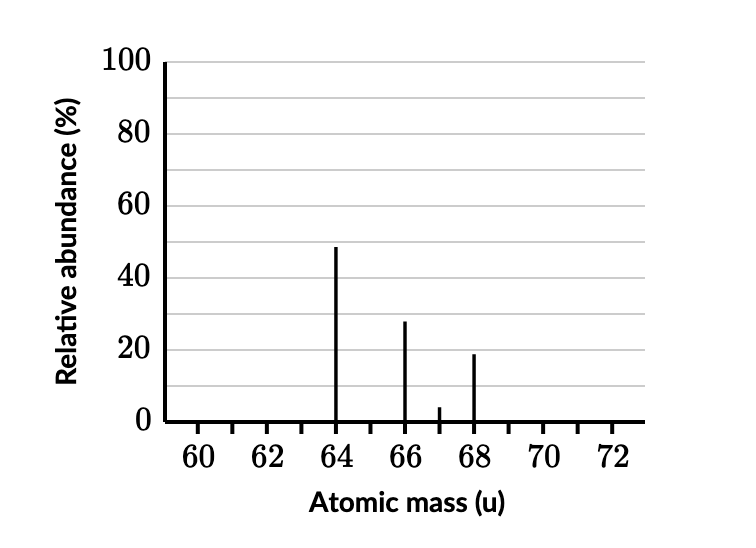
\includegraphics[scale = 0.5]{photos/photo1.png}
\end{center}
(a) In an average sample of the element, less than \(20\%\) of the atoms have an atomic mass of \(66u\). \\
(b) The most abundant isotope of the element has an atomic mass of \(64u\). \\
(c) The element has an average atomic mass of \(64u\). \\
(d) The element has an average atomic mass between \(66\) and \(68u\). \\
\subsection*{Problem \countThis}
What is the percent composition of Carbon in \(\ce{C_{13}H_{18}O_2}\)?
\subsection*{Problem \countThis}
A compound contains \(32.38\%\) sodium, \(22.65\%\) sulfur, and \(44.99\%\) oxygen. What is the emperical forumula. 
\subsection*{Problem \countThis}
What is the full electron configuration of mercury?
\subsection*{Problem \countThis}
Below, the photoelectron spectra of the \(2s\) electrons of \(\ce{Be}\) and \(\ce{Mg}\) are shown.
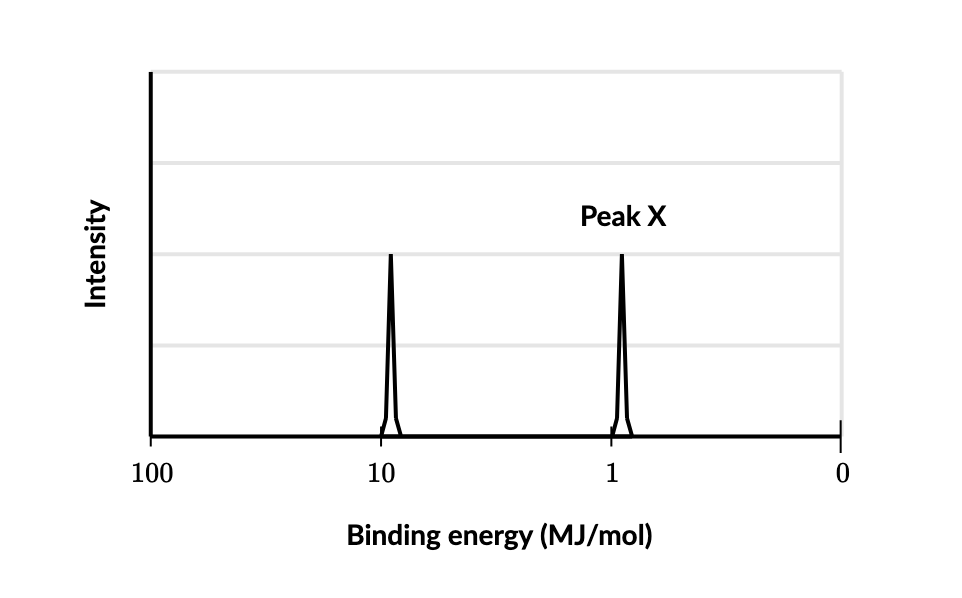
\includegraphics[scale = 0.5]{photos/photo2.png} \\
Is peak \(X\) the peak associated with \(\ce{Be}\) or \(\ce{Mg}\)?
\subsection*{Problem \countThis}
What are the periodic trends of ionization energy, atomic radius, and electronegativity? Why?
\section{Unit 2: Molecular and Ionic Compound Structure and Properties}
\subsection*{Problem \countThis}
Which of the following bonds is likely to have the most ionic character? \\
(a) \chemfig{H-F} \\
(b) \chemfig{C-O} \\
(c) \chemfig{Na-F}\\
(d) \chemfig{Mg-O}
\subsection*{Problem \countThis}
Based on the information in the table, which of the following arranges the bonds in order of decreasing polarity? \\
\begin{center}
\begin{tabular}{|cc|}
    \hline 
    Element & Electronegativity \\ [0.5 ex]
    \hline \hline
    \(\ce{H}\) & \(2.2\)\\
    \(\ce{N}\) & \(3.0\) \\
    \(\ce{F}\) & \(4.0\) \\
    \(\ce{Cl}\) & \(3.2\) \\
    \(\ce{Se}\) & \(2.6\) \\
    \(\ce{I}\) & \(2.7\)\\ [1ex]
    \hline
\end{tabular}
\end{center} 
(a) \(\chemfig{Se-N} > \chemfig{H-I} > \chemfig{Cl-F}\) \\
(b) \(\chemfig{H-I} > \chemfig{Se-N} >\chemfig{Cl-F}\)\\
(c) \(\chemfig{Cl-F} > \chemfig{H-I} > \chemfig{Se-N}\)\\
(d) \(\chemfig{Cl-F} > \chemfig{Se-N} > \chemfig{H-I}\)
\subsection*{Problem \countThis}
Why is the lattice energy of \ce{CsF} smaller than the lattice energy of \ce{KF}?
\subsection*{Problem \countThis}
What type of structure do metallic elements form and through what bonds? 
\subsection*{Problem \countThis}
What are the two types of metallic alloys and what are there differences?
\subsection*{Problem \countThis}
Draw a Lewis Diagram for Acetic Acid \ce{CH3COOH}.
\subsection*{Problem \countThis}
Draw the Lewis Diagram for \ce{CO2}
\subsection*{Problem \countThis}
Draw the Lewis Diagram(s) for ozone, \ce{O3}
\ProblemSet
Write the formal charges for all three molecules above.
\ProblemSet
What is the electron geometry, molecular geometry, and hybridization of the central atom in this molecule. \\ 
\chemfig{\charge{-90=\:}{N}(-[:90]H)(-[:225]H)(-[:315]H)}
\ProblemSet
What are the intermolecular forces present among these molecules. \\ 
\chemfig{H-C(-[:-90]H)(-[:90]H)-C(=[:90]O)-O-C(-[:90]H)(-[:-90]H)-H}
\ProblemSet
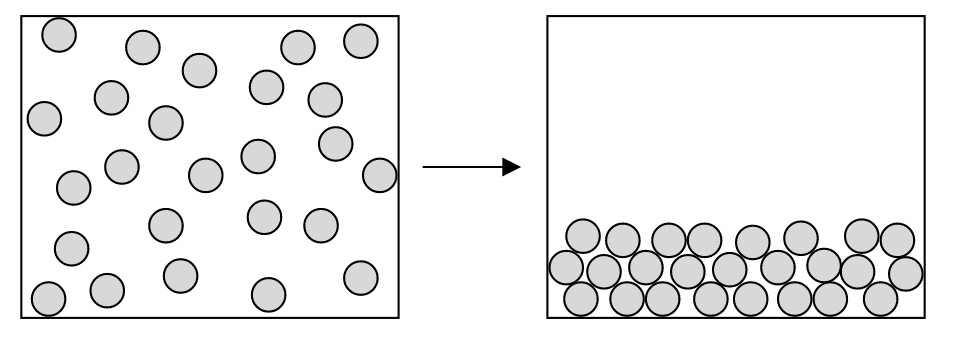
\includegraphics[scale = 0.5]{photo3.png}
What phase transition is this?
\ProblemSet
Originally, a sample of gas is in a rigid container at \(299K\) and \(0.70 atm\). The student increases the temperature of the \ce{CO2(g)} in the container to \(425K\).\\
(a) What does raising the temperature do to the mostion of the molecules?\\
(b) What is the pressure at \(425K\)?\\
(c) In terms of Kinetic Molecular Theory, why does the pressure of gas change as it is heated? \\
\ProblemSet
A \(60.3g\) of \ce{Be(OH)2} is dissolved in enough water to produce \(1.75L\) of solution. Calculate the concentration of \ce{OH-} ions. 


\setcounter{yayCounter}{1}
\newpage
\section{Answers}
\subsection{Unit 1}
\subsubsection*{Problem \countThis}
The molar mass of \(\ce{C_9H_8O_4}\) is \(1.008*8 + 12.01*9 + 16.00*4 = 180.2 \frac{g}{mol}\)
\begin{equation}
\begin{aligned}
    7.89kg \times \frac{1g}{10^{-3}kg} \times \frac{1mol}{180.2g} = 43.8mol
\end{aligned}
\end{equation}
\subsubsection*{Problem \countThis}
(b), the tallest peak of the graph is the one at \(64u\). 
\subsubsection*{Problem \countThis}
In one mole of \(\ce{C_{13}H_{18}O_2}\) is \(206.31g\).
\begin{equation}
\begin{aligned}
    1mol\hspace{0.1em}\ce{C_{13}H_{18}O_2} \times \frac{13mol\hspace{0.1em}\ce{C}}{1mol\ce{C_{13}H_{18}O_2}} \times \frac{12.01g}{1mol\hspace{0.1em}\ce{C}} = 156.31g
\end{aligned}
\end{equation}
Thus, the percent composition by weight is \(\frac{156.31}{206.31} = 75.764\%\)
\subsubsection*{Problem \countThis}
Take \(100g\) of the substance such that there are \(32.38g\) sodium, \(22.65g\) sulfur, and \(44.99g\) oxygen. 
\begin{equation}
\begin{aligned}
    32.38g\hspace{0.1em}\ce{Na} \times \frac{1mol\hspace{0.1em}\ce{Na}}{22.99g} &= 1.408mol\hspace{0.1em}\ce{Na} \\
    22.65\hspace{0.2em}g \ce{S} * \frac{1\hspace{0.2em}mol\ce{S}}{32.07g} &= 0.7063 \hspace{0.2em}mol\ce{S}\\
    44.99\hspace{0.2em}g\ce{O} * \frac{1\hspace{0.2em}mol\ce{O}}{16 g} &= 2.812\hspace{0.2em}mol \ce{O}
\end{aligned}
\end{equation}
Take the ratio of each compound with the smallest quantity. 
\begin{equation}
\begin{split}
    S:\hspace{0.2em}\frac{0.7063}{0.7063} = 1 \\
    Na:\hspace{0.2em}\frac{1.408}{0.7063} = 2 \\
    O:\hspace{0.2em}\frac{2.812}{0.7063} = 4
\end{split}
\end{equation}
Therefore, the empirical formula is \(Na_{2}SO_{4}\)
\subsubsection*{Problem \countThis}
\(1s^22s^22p^63s^23p^64s^23d^{10}4p^65s^24d^{10}5p^66s^24f^{14}5d^{10}\)
\subsubsection*{Problem \countThis}
\(\ce{Be}\). The peak location of the peak on the x-axis means that there is less binding energy for the electrons in element \(X\). \(\ce{Be}\) has fewer protons
and both electrons are in the same shell, so it peak must belong to \(\ce{Be}\).
\subsubsection*{Problem \countThis}
\begin{itemize}
\item The electronegativity increases from left to right across a period. This is because if a valence shell of electrons is less than half full than
it requires less energy to lose an electron than gain one. If if the valence shell of electrons is more than half full, it is easier to pull and electron
into the valence shell. The electronegativity decreases from the top to the bottom of a group. This is beause there is a greater atomic radius lower on the group.

\item The ionization energy increases from left to right in a period. This is because of greater valence shell stability also because of smaller atomic radius. The ionization energy also decreases
from top to bottom of a group. This is because of greater electron shielding and greater atomic radius. 

\item Atomic radius decreases from left to right within a period. This is because there are more protons to the right of the period. Atomic radius increases from top to bottom within a group.
 This is because of electron shielding and there are more electron shells in the atom. 
\end{itemize}  
\subsection{Unit 2}
\subsubsection*{Problem \countThis}
The ionic character increase the greater the electronegativity difference. In this case, \(\ce{Na}\) and \(\ce{O}\) had the greatest electronegativity difference. 
\subsubsection*{Problem \countThis}
(c) \(\chemfig{Cl-F} > \chemfig{H-I} > \chemfig{Se-N}\)
\subsubsection*{Problem \countThis}
\ce{Cs+} has a larger atomic radius than \ce{K+}. So the distance between the cation and anion is greater than in \ce{CsF} than in \ce{KF}
\subsubsection*{Problem \countThis}
Most metallic elements form crystalline solids at room temperature. Their bonds are metallic bonds due to electrostatic attraction between metal cations and delocalized electrons. 
\subsubsection*{Problem \countThis}
\begin{itemize}
    \item Substitutional alloys. These alloys form when one atom of a similar size to the host metal replaces an atom of the host metal. The substitute atom must be of similar size. These alloys have good thermal and electrical conductivity.
    \item Interstitial alloys. These alloys are formed when smaller atoms fill in the gaps between the larger host atoms. This makes the metal harder and less malleable. 
\end{itemize}
\subsubsection*{Problem \countThis}
\chemfig{H-C(-[:90]H)(-[:270]H)-C(=[:90]\charge{180=\:, 0 = \:}{O})-\charge{90 =\:, -90 =\:}{O}-H}
\subsubsection*{Problem \countThis}
\chemfig{\charge{90=\:,-90=\:}{O}=C=\charge{90 =\:, -90=\:}{O}}
\subsubsection*{Problem \countThis}
\chemfig{\charge{90=\:}{O}(=[:330]\charge{60=\:,240=\:}{O})(-[:210]\charge{120=\:, 315=\:, 225=\:}{O})}
\(\longleftrightarrow\)
\chemfig{\charge{90=\:}{O}(=[:210]\charge{135=\:,315=\:}{O})(-[:330]\charge{45=\:, 315=\:, 225=\:}{O})}
\AnswerSet
All formal charges of \ce{CH3COOH} and \ce{CO2} are zero. \\
\chemfig{O^{+1}(=[:330]O)(-[:210]O^{-1})}
\(\longleftrightarrow\)
\chemfig{O^{+1}(=[:210]O)(-[:330]O^{-1})}
\AnswerSet
The electron geometry is tetrahedral. The molecular geometry is trigonal pyramidal. Hybridization of \ce{N} atom is \(sp^3\) since it has tetrahedral electron geometry.
\AnswerSet
Dipole-diple and london dispersion forces. The \chemfig{C-O} bond is polar and the molecule is asymmetrical so it is polar. There are no \chemfig{H-F}, \chemfig{H-O}, or \chemfig{H-N} bonds, so there is no hydrogen bonding. 
\AnswerSet
Condensation. Both have no regular arrangement, the one on the left is separated by the one on the right is close together, so the molecules are transitioning from gas to liquid.
\AnswerSet
(a) As you increase the temperature, the average kinetic energy or speed increases as well. \\
(b) \(n_1 = n_2\) and \(V_1 = V_2\), so \(P_1V_1 = n_1RT_1\) and \(P_2V_2 = n_2RT_2\). \(\frac{P_2V_2}{RT_2} = \frac{P_1V_1}{RT_1} \implies P_2 = \frac{P_1T_2}{T_1} = \frac{0.7 * 425}{299} = 0.99atm\)\\
(c) As the temperature increases, the average kinetic energy increases, so the molecules undergo more collisions with the walls of the container.  \\
\AnswerSet
\begin{equation*}
    60.3g \times \frac{1mol\hspace{0.2em}\ce{Ba(OH)2}}{171.35g} \times \frac{2mol\hspace{0.2em}\ce{OH-}}{1mol\hspace{0.2em}\ce{Ba(OH)2}} * \frac{1}{1.75L} = 0.402M
\end{equation*}

\end{document}